% Figure from MATH 556 notes, section 14. Compile with the notes preamble.
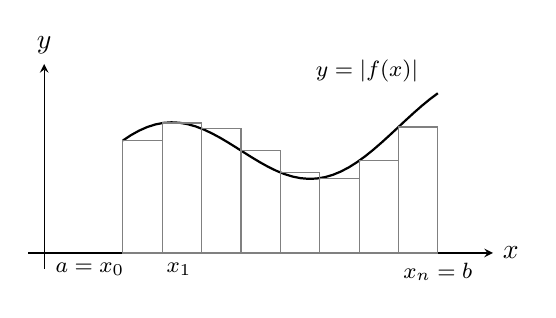
\begin{tikzpicture}[scale=1.0, >=stealth]
    \draw[->] (-0.7,0) -- (5.2,0) node[right] {$x$};
    \draw[->] (-0.5,-0.2) -- (-0.5,2.4) node[above] {$y$};
    \draw[thick, domain=0.5:4.5, samples=40] plot (\x, {1.0 + 0.5*sin(\x*90) + 0.15*\x});
    \node[above, font=\footnotesize] at (3.6,2.05) {$y = |f(x)|$};
    \foreach \i in {0,...,7} {
        \pgfmathsetmacro{\xa}{0.5 + \i*0.5}
        \pgfmathsetmacro{\ya}{1.0 + 0.5*sin(\xa*90) + 0.15*\xa}
        \draw[thin, gray] (\xa,0) rectangle ({\xa+0.5},\ya);
    }
    \node[below, font=\footnotesize, anchor=north east, xshift=4pt] at (0.5,0) {$a = x_0$};
    \node[below, font=\footnotesize, anchor=north west, xshift=-2pt] at (1.0,0) {$x_1$};
    \node[below, font=\footnotesize] at (4.5,0) {$x_n = b$};
\end{tikzpicture}
